\documentclass{standalone}
%\pagenumbering{gobble}


%%%%%%%%%%%%%%%%%%%%%%%%%%%%%%%%%%%%%%%%%%%%
% shock schematic
%
%%%%%%%%%%%%%%%%%%%%%%%%%%%%%%%%%%%%%%%%%%%%


\usepackage{tikz,xcolor}
\usetikzlibrary{arrows, shadings, calc}

\begin{document}

\tikzset{
	level/.style={thick},
	trans/.style={thick, dashed,->,shorten >=2pt,shorten <=2pt,>=stealth},
	photon/.style={thick, ->, snake=snake, line after snake=1mm}
	}


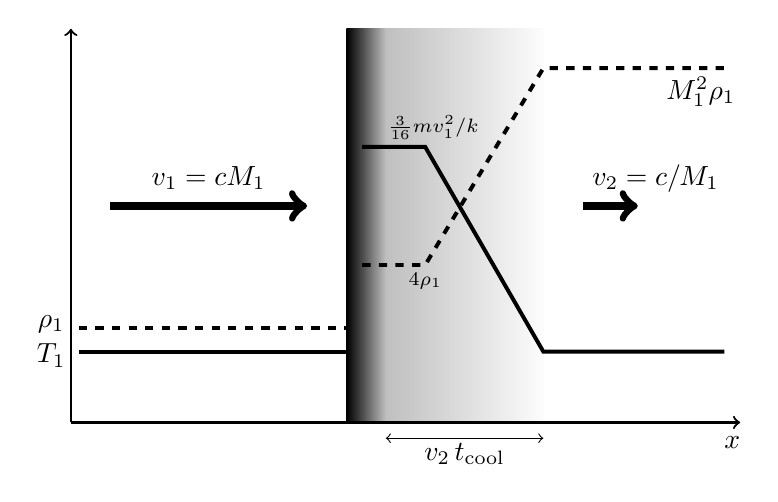
\begin{tikzpicture}[scale=1.0, font=\sffamily]

	% shaded area for shock
	\begin{scope}%[transform canvas={rotate=30}]
		\shade[shading=axis,bottom color=black,top color=gray!50, shading angle=-90] (3.5,0) rectangle (4.0,5);
		\shade[shading=axis,bottom color=gray!50,top color=gray!2, shading angle=-90] (4.0,0) rectangle (6.0,5);
	\end{scope}

	% velocity
	\draw[thick, line width=1mm, ->] (0.5,2.75) -- (3.0,2.75);
	\node at (1.75, 3.1) {$v_1 = cM_1$};
	\draw[thick, line width=1mm, ->] (6.5,2.75) -- (7.2,2.75);
	\node[right] at (6.5, 3.1) {$v_2 = c/M_1$};

	% temperature
	\node at (-0.25, 0.85) {$T_1$};
	\draw[line width = 0.5mm] (0.1,0.9) -- (3.5,0.9);
	\draw[line width = 0.5mm] plot [smooth, tension=0] coordinates {(3.7,3.5) (4.5,3.5) (6.0,0.9) (8.3, 0.9)};
	\node at (4.6, 3.75) {\scriptsize{$\frac{3}{16}mv_1^2/k$}};

	% density
	\node at (-0.25, 1.25) {$\rho_1$};
	\draw[line width = 0.5mm, dashed] (0.1,1.2) -- (3.5,1.2);
	\draw[line width = 0.5mm, dashed] plot [smooth, tension=0] coordinates {(3.7,2.0) (4.5,2.0) (6.0,4.5) (8.3, 4.5)};
	\node at (4.5, 1.8) {\scriptsize{$4\rho_1$}};
	\node at (8.0, 4.2) {$M_1^2\rho_1$};

	% axes
	\draw[thick, ->] (0,0) -- (8.5,0);
	\draw[thick, ->] (0,0) -- (0,5);
	\node at (8.4, -0.25) {$x$};
	%\node at (-0.2, 5) {$T, \rho$};
	\draw[<->] (4.0,-0.2) -- (6.0,-0.2);
	\node at (5.0,-0.4) {$v_2\,t_{\rm cool}$};

\end{tikzpicture}

\end{document} 
